Si precisa che tutti in tutti gli scenari simulati si assume che la rete sia completamente connessa per cui da un qualsiasi nodo \textit{x} è possibile raggiungere tramite uno o più nodi il nodo \textit{sink}.
\\\\
\textit{1) TX Time}: come mostrato in \textbf{Figura \ref{fig:TXTime_final2.0}}, si è riusciti a migliorare ulteriormente l'invio di pacchetti di wake-up rispetto la normale \textit{All-in-One}. Ovviamente questo miglioramento si ha in quanto essendo dinamico il tempo per cui si usa il caching di un relay e dato che il tetto massimo è maggiore del numero usato nella prima versione di \textit{All-in-One} ci saranno sicuramente meno fasi di Relay-Selection.\\
In particolare si osserva un miglioramento di circa il 47\% rispetto la prima versione di \textit{All-in-One}.
\\\\
\textit{2) Energy Consuption}: come mostrato in \textbf{Figura \ref{fig:EnergySpent_final2.0}}, la gestione dinamica del numero di ritrasmissioni e il Jitter basato sull'energia residua comportano un miglioramento anche nell'energia complessiva consumata dalla rete. Anche qui si ha un miglioramento del 5\% circa, dovuto al fatto che i vari nodi potrebbero evitare molte più volte la fase di Relay-Selection, avviandola solo nei casi in cui il nodo cached potrebbe scaricarsi.
\\\\
\textit{3) End-to-End Latency}: come mostrato in \textbf{Figura \ref{fig:Latency_final2.0}}, anche il ritardo End-to-End migliora rispetto la versione base. Ovviamente gestendo meglio l'energia consumata e non vincolando l'uso del nodo cached a 3 ma riducendolo o aumentandolo a seconda dei casi ci saranno meno ritrasmissioni dovuti a nodi non più disponibili oltre che meno scambi di pacchetti dovuti alla fase di Relay-Selection. \\
In particolare, anche qui, i miglioramenti sono circa del 5-6\% in tutte le varie configurazioni.
\\\\
\textit{4) Packet Delivery Ratio}: come mostrato in \textbf{Figura \ref{fig:PDR_final2.0}}, la percentuale dei pacchetti ricevuti, che era un punto debole della prima versione di \textit{All-in-One}, è migliorata molto. Si ottiene infatti sempre tra il 99.9\% e il 100\% dei pacchetti consegnati, perdendone circa in quantità minime come 2 o 3 solitamente. \\
Gestendo meglio l'energia ci saranno sempre meno nodi indisponibili per cui le probabilità di perdita dei pacchetti diminuiscono.

\begin{figure}[H]
  \begin{subfigure}[t]{0.49\linewidth}
    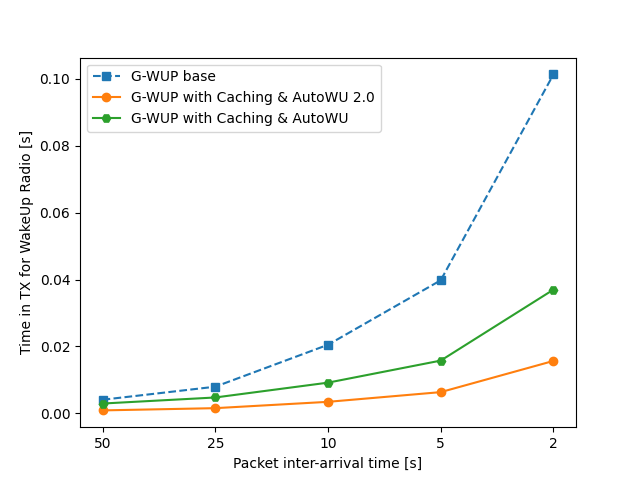
\includegraphics[width=1.1\linewidth]{Contents/Images/graphs/final2.0/tx_time.png}
    \caption{TX Time for the WUR}
    \label{fig:TXTime_final2.0}
  \end{subfigure}
  \begin{subfigure}[t]{0.49\linewidth}
    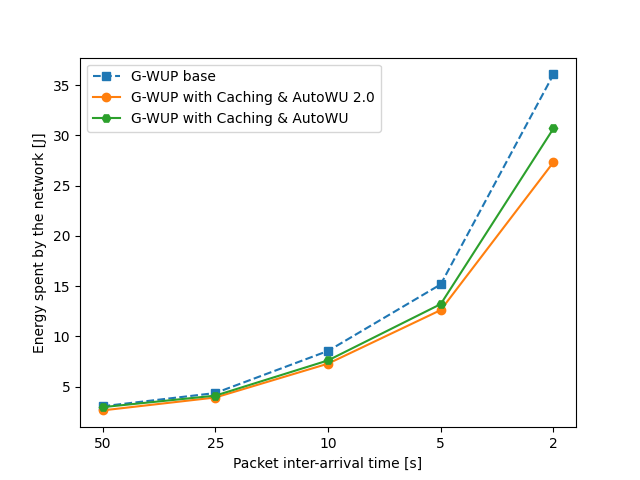
\includegraphics[width=1.1\linewidth]{Contents/Images/graphs/final2.0/energySpent.png}
    \caption{Energy Consuption}
    \label{fig:EnergySpent_final2.0}
  \end{subfigure}
  \begin{subfigure}[t]{0.49\linewidth}
    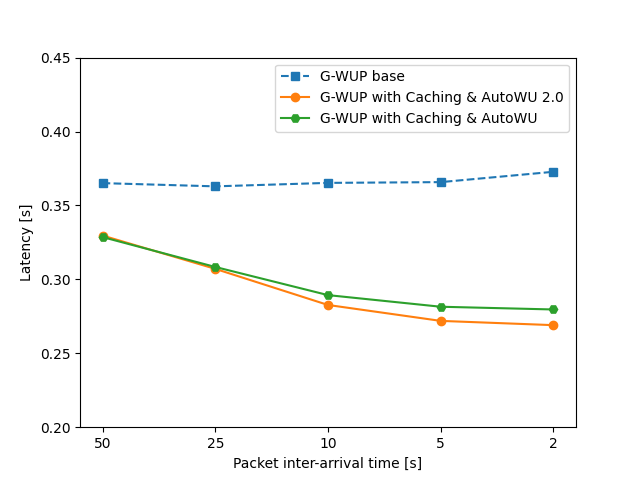
\includegraphics[width=1.1\linewidth]{Contents/Images/graphs/final2.0/latency.png}
    \caption{End-to-End Latency}
    \label{fig:Latency_final2.0}
  \end{subfigure}
  \begin{subfigure}[t]{0.49\linewidth}
    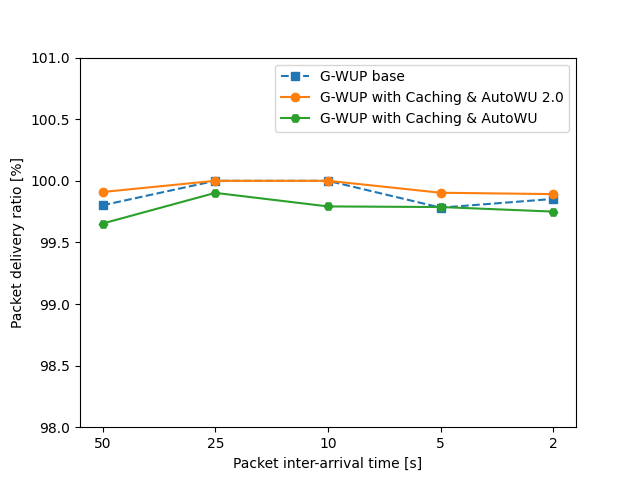
\includegraphics[width=1.1\linewidth]{Contents/Images/graphs/final2.0/pdr.png}
    \caption{Packet Delivery Ratio}
    \label{fig:PDR_final2.0}
  \end{subfigure}
  \caption{Confronto delle prestazioni tra versione base di GreenWUP (blu) e le varianti proposte}
  \label{fig:final2.0}
\end{figure}

La combinazione di tutti i meccanismi proposti consente netti miglioramenti in termini di tutte le metriche prestazionali rispetto al protocollo base. E' efficace nel ridurre al minimo gli onerosi scambi di pacchetti di controllo, consente la scelta dei migliori relay. Questo migliora le prestazioni in termini anche di packet delivery ratio e latenza.